\chapter{Solución}
\section{¿Por qué Ruby on Rails?}

Para responder a esta pregunta, es necesario primero definir a \textbf{Ruby on Rails}, llamado tambien \emph{Rails} ó RoR, es un \emph{framework} que hace que sea más fácil desarrollar, implementar, y mantener aplicaciones web. Durante los meses que siguieron a su primera liberación, \emph{Rails} paso de ser un juguete desconocido a un fenomeno mundial. Ha ganado premios, y más importante aún, se ha convertido en el framework de preferencia para la implementación de cierto conjunto de las llamadas aplicaciones Web 2.0\cite{ror:awdwr}.\\

Se eligió \emph{Rails} para desarrollar la aplicación web en la que se comunican datos y contenidos 3D, por qué se buscaba utilizar una herramienta en la que la convención estuviera por encima de la configuración\footnote{Léase \textbf{CoC} en el glosario}, que contará con una arquitectura pre definida, en éste caso MVC (Modelo Vista Controlador) Figura\ref{fig:mvc} que \emph{Rails} aprovecha apropiadamente, cuándo se desarrolla en \emph{Rails}, hay un lugar para cada pieza de código\footnote{Léase \textbf{DRY} en el glosario}, y todos los componentes de la aplicación interactúan según el estándar.\\

\begin{figure}[h]
	\centering
		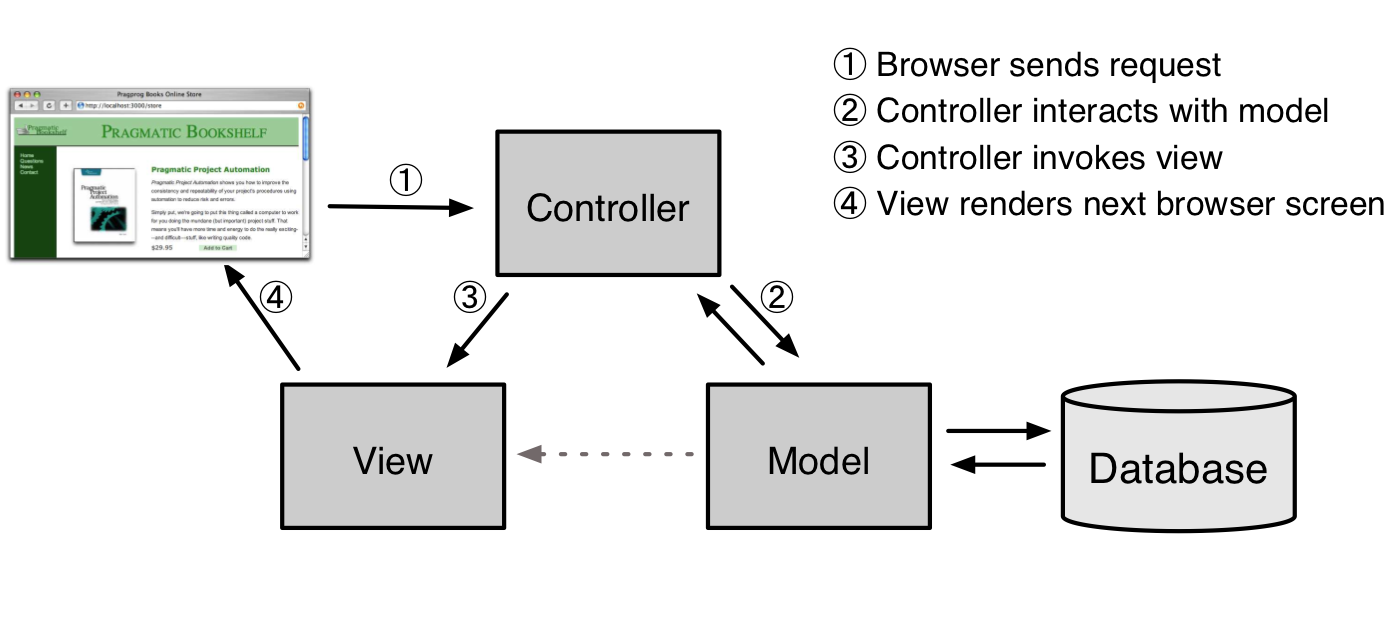
\includegraphics[scale=0.25]{mvc.PNG}
		\caption{Modelo Vista Controlador}
	\label{fig:mvc}
\end{figure}

Los programadores profesionales, suelen escribir tests para simular el comportamiento de la aplicación que se esta desarrollando, para el presente proyecto, se buscaba que el framework tuvieran un soporte para hacer tests, una vez más Rails se ajusta a esas necesidades, pues cuenta con soporte para algunos frameworks para realizar tests, se encuentran; RSpec (utilizada en este proyecto, bajo la filosofía de TDD \footnote{Léase \textbf{TDD} en el glosario}) en donde se escriben los tests, antes de la implementación, Test Unit, Shoulda y Cucumber (BDD\footnote{Léase \textbf{BDD} en el glosario})\\

Se buscaba que la herramienta fuera escrita en un lenguaje de programación orientado a objetos e interpretado, por la necesidad de crear \emph{scripts} que corrieran independiente de la aplicación, como tareas programadas para correr cada cierto tiempo. Las aplicaciones en \emph{Rails} son escritas en el lenguaje de programación \emph{Ruby}, que cumple con lo que se buscaba, y aparte introduce características favorables como metaprogramación, haciendo que el código sea más fácil de entender, leer y/o escribir, programas más cortos en términos de \textbf{LOC}\footnote{Líneas de código, en inglés \emph{Lines of Code}}, para evidenciar esto, a continuación se muestra una porción de código de la aplicación, en la que se define una clase de un Modelo que expresa mucha información en pocas líneas de código y es fácil de entender. \\

codigo aca \\

Finalmente, no se pretendía manipular la base de datos directamente, es decir, con código nativo del motor de bases de datos, sino sacar provecho de técnicas como ORM \footnote{Léase \textbf{ORM} en el glosario}, en las que las tablas de las bases de datos son mapeadas a clases, los registros de las tablas son mapeados como objetos, y consecuentemente los campos, se mapean como atributos de los objetos, mientras que existen metodos de clases que se encargan de realizar operaciones a nivel de tablas, dejando como opcional la utilización de código \textbf{SQL} dentro de la aplicación, una vez más \emph{Rails} suple esta necesidad con \textbf{ActiveRecord} ó \textbf{Datamapper}.